\documentclass[10pt]{article}

\usepackage[letterpaper,margin=0.68in,top=0.74in,bottom=0.78in]{geometry}
\usepackage{microtype}
\usepackage{fancyhdr}
\usepackage[table]{xcolor}
\usepackage{tikz}
\usetikzlibrary{positioning}
\usepackage{multicol}
\usepackage{tabularx}
\usepackage{array}
\usepackage{longtable}
\usepackage{caption}
\usepackage{needspace}
\usepackage{hyperref}

\definecolor{panel}{RGB}{255,246,214}
\definecolor{tabhead}{RGB}{250,214,202}
\definecolor{boxblue}{RGB}{214,228,242}
\definecolor{boxrose}{RGB}{246,220,220}
\definecolor{boxline}{RGB}{48,79,120}

\hypersetup{
  colorlinks=true,
  urlcolor=black,
  linkcolor=black,
  pdftitle={wavves for IST 688},
  pdfauthor={Gil Raitses}
}

\captionsetup{font=small,labelfont=bf,labelsep=period,skip=3pt}
\setlength{\parskip}{0.25em}
\setlength{\parindent}{1.15em}
\setlength{\headheight}{14pt}
\setlength{\columnsep}{0.85em}
\emergencystretch=1.5em
\urlstyle{same}

\pagestyle{fancy}
\fancyhf{}
\fancyhead[L]{wavves for IST 688}
\fancyhead[R]{Gil Raitses}
\renewcommand{\headrulewidth}{0.4pt}
\fancyfoot[L]{\footnotesize IST 688 Building Human-Centered AI Applications}
\fancyfoot[R]{\footnotesize\begin{tabular}[b]{@{}r@{}}November 6, 2026\\Prof. Jeffrey Saltz\end{tabular}}
\renewcommand{\footrulewidth}{0.4pt}

\newcommand{\sect}[1]{%
  \par\addvspace{0.75em}%
  \noindent{\normalsize\bfseries #1}\par\nopagebreak
  \addvspace{0.2em}%
  \noindent\ignorespaces
}

\newcommand{\panel}[1]{%
  \par\medskip\noindent
  \colorbox{panel}{%
    \begin{minipage}{\dimexpr\linewidth-2\fboxsep\relax}
      \smallskip
      #1
      \smallskip
    \end{minipage}%
  }%
  \par\medskip
}

\tikzset{
  filebox/.style={
    draw=boxline,
    rounded corners=2pt,
    fill=white,
    font=\footnotesize\ttfamily,
    align=center,
    inner sep=4pt,
    text=black
  },
  stepbox/.style={
    draw=boxline,
    rounded corners=2pt,
    fill=boxblue,
    font=\footnotesize,
    align=center,
    inner sep=4pt,
    text width=1.42in
  },
  stepboxb/.style={
    draw=boxline,
    rounded corners=2pt,
    fill=boxrose,
    font=\footnotesize,
    align=center,
    inner sep=4pt,
    text width=1.42in
  }
}

\begin{document}

\begin{center}
{\large\bfseries Short Requests, Saved Files and a Later Check\par}
\vspace{0.25em}
{\normalsize A class reading from the public wavves pages and the repository README\par}
\end{center}

\begin{multicols}{2}
A person starts with a short request. The repository README says the \texttt{/wavves} entry reads the request, checks the home, picks a playbook and runs that skill.\footnote{Repository README in this repo, version line 0.5.0.} The published examples are short tasks in ordinary language.

The public listing describes a worked session on that entry.\footnote{\url{https://www.agensi.io/skills/wavves}} The request charters a lane named docs-sweep for a public docs refresh and runs a first \texttt{/mod-check} on the written plan. The moderator wrote \texttt{waveset.md} under the lane home. Parallel runners in that review wave returned blockers along with gaps. The build step stayed unstarted during the open review wave.

The class has been talking about a context window that fills up and about recaps that drop detail. The listing answers the window problem this way. A person charters lanes so long work runs as waves with state saved on disk. An orchestration agent runs the waves in the background. Runners do the scoped execution-layer work assigned by that agent. The next moderator term hydrates from files on disk with nothing carried over in the context window.

The class pattern is a short live window plus lasting files, with a later check before the next stretch opens. The later check is \texttt{/remeasure} on the JSON and the log in \texttt{gate-captures}. On pickup the next term also runs the pickup check and can run the rotation history audit. The public site describes that same folder layout and says the control-surface video uses invented sample files.\footnote{\url{https://wavves.aimez.ai/}}
\end{multicols}

\panel{%
\begin{center}
\textbf{Files a Fresh Term Reads}
\end{center}
\vspace{0.15em}
\begin{center}
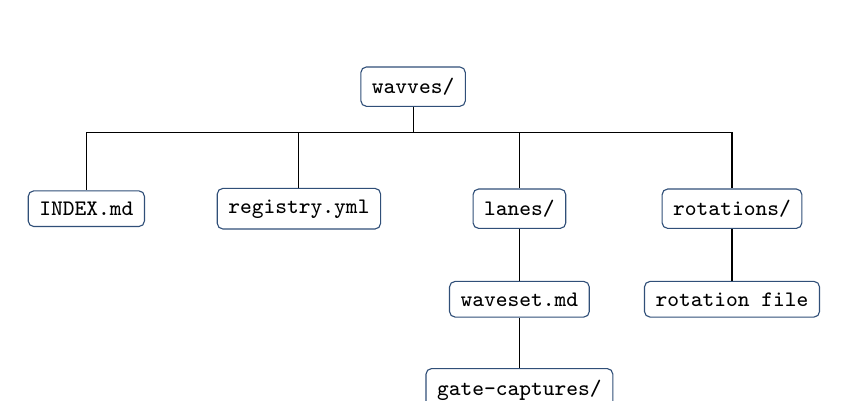
\begin{tikzpicture}[x=1cm,y=1cm]
  \node[filebox] (home) at (0,0) {wavves/};
  \node[filebox] (index) at (-4.15,-1.55) {INDEX.md};
  \node[filebox] (reg) at (-1.45,-1.55) {registry.yml};
  \node[filebox] (lanes) at (1.35,-1.55) {lanes/};
  \node[filebox] (rots) at (4.05,-1.55) {rotations/};
  \node[filebox] (wave) at (1.35,-2.7) {waveset.md};
  \node[filebox] (gate) at (1.35,-3.85) {gate-captures/};
  \node[filebox] (rot) at (4.05,-2.7) {rotation file};
  \draw (home.south) -- ++(0,-0.32) coordinate (bus);
  \draw (bus) -| (index.north);
  \draw (bus) -| (reg.north);
  \draw (bus) -| (lanes.north);
  \draw (bus) -| (rots.north);
  \draw (lanes.south) -- (wave.north);
  \draw (wave.south) -- (gate.north);
  \draw (rots.south) -- (rot.north);
\end{tikzpicture}
\end{center}
\captionof{figure}{Home files named across the sources. The public site shows \texttt{INDEX.md}, lane folders, a waveset, \texttt{gate-captures} and a rotations folder. The README adds \texttt{registry.yml}, \texttt{AGENTS.md}, \texttt{step-log.md}, dispatch files, \texttt{findings/} and \texttt{decisions/}. Lines show which folder holds which file. The site says the demo sample files are invented.}
}

\panel{%
\begin{center}
\textbf{Two Orders the Sources Actually Give}
\end{center}
\vspace{0.35em}
\begin{center}
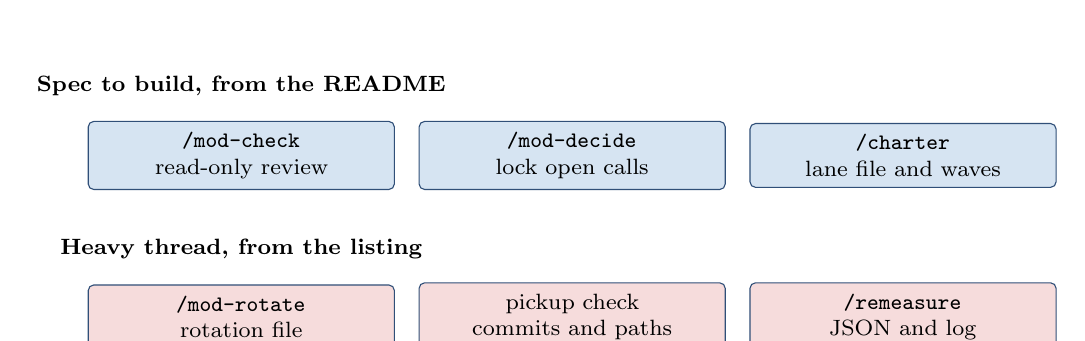
\begin{tikzpicture}[node distance=3mm]
  \node[font=\footnotesize\bfseries] (h1) {Spec to build, from the README};
  \node[stepbox, below=2mm of h1] (a) {\texttt{/mod-check}\\read-only review};
  \node[stepbox, right=3mm of a] (b) {\texttt{/mod-decide}\\lock open calls};
  \node[stepbox, right=3mm of b] (c) {\texttt{/charter}\\lane file and waves};
  \node[font=\footnotesize\bfseries, below=5mm of a] (h2) {Heavy thread, from the listing};
  \node[stepboxb, below=2mm of h2] (d) {\texttt{/mod-rotate}\\rotation file};
  \node[stepboxb, right=3mm of d] (e) {pickup check\\commits and paths};
  \node[stepboxb, right=3mm of e] (f) {\texttt{/remeasure}\\JSON and log};
\end{tikzpicture}
\end{center}
\captionof{figure}{Left to right within each row. The README gives the spec to build order as \texttt{/mod-check}, then \texttt{/mod-decide}, then \texttt{/charter}. The listing gives the heavy-thread order as a rotation file, then the pickup check, then a remeasure of \texttt{gate-captures}. These are two sourced orders. The docs-sweep session left the build step unstarted while the review wave was open.}
}

\panel{%
\begin{center}
\textbf{What a Pickup Reads}
\end{center}
\vspace{0.35em}
\begin{center}
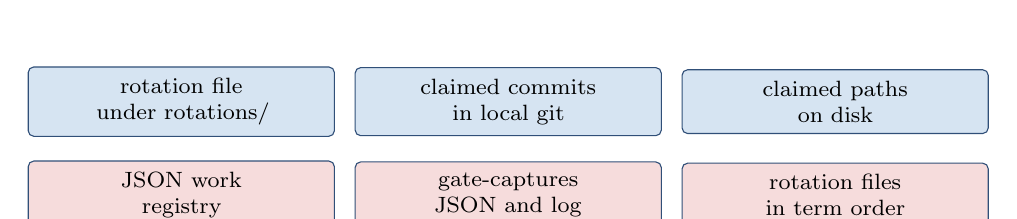
\begin{tikzpicture}[node distance=2.5mm]
  \node[stepbox] (a) {rotation file\\under rotations/};
  \node[stepbox, right=2.5mm of a] (b) {claimed commits\\in local git};
  \node[stepbox, right=2.5mm of b] (c) {claimed paths\\on disk};
  \node[stepboxb, below=3mm of a] (d) {JSON work\\registry};
  \node[stepboxb, right=2.5mm of d] (e) {gate-captures\\JSON and log};
  \node[stepboxb, right=2.5mm of e] (f) {rotation files\\in term order};
\end{tikzpicture}
\end{center}
\captionof{figure}{The listing says one pickup script tests claimed commits against local git and looks for claimed paths. A second check covers the JSON work registry. The same pickup remeasures \texttt{gate-captures}. The rotation history audit then reads rotation files in order. A fix row for script messages sits in five recovery playbooks.}
}

\sect{Published usage}

The listing's example session prompt is a short request.

\begin{quote}
\ttfamily
/wavves charter a lane named docs-sweep\\
for the public docs refresh\\
and run a first /mod-check on the written plan
\end{quote}

\noindent The listing says that session chartered the lane, wrote \texttt{waveset.md}, ran a read-only review wave and left the build step unstarted.

The README prints prompt shapes for the same skills. It also says the paths and metrics in \texttt{examples/usage.md} are fictional. That file is not in this repository. The lines below are prompt shapes from the README, not measured runs.

\begin{quote}
\ttfamily
/wavves set up in this repo, then audit our README for drift.\\
/mod-check the landed spec.\\
/mod-decide lock the open calls.\\
/wavves hydrate from the rotation paste and tell me what's active.
\end{quote}

\noindent Leaf skills from the README. The listing also names \texttt{/remeasure}, which the README skill table does not use.

\begin{center}
\small
\begin{tabular}{@{}ll@{}}
\hline
\rowcolor{tabhead}
Skill & When the sources say to use it \\
\hline
\texttt{/wavves} & Default entry. Matches a playbook and runs it. \\
\texttt{/wavves-init} & Home setup only. \\
\texttt{/charter} & Charter a lane and dispatch waves behind gates. \\
\texttt{/mod-check} & Read-only review of a landed spec or plan. \\
\texttt{/mod-decide} & Lock open calls before a build charter. \\
\texttt{/layover} & Read-only audit of a multi-root workspace. \\
\texttt{/mod-rotate} & Hand a heavy thread to the next moderator term. \\
\texttt{/mod-kick} & Move to another machine with an allowlist and a short paste. \\
\texttt{/shrug} & Carry out recommended actions from a verdict. \\
\texttt{/remeasure} & Listing name for turning a done claim into a rerunnable gate. \\
\hline
\end{tabular}
\end{center}
\captionof{table}{Skills named in the repository README, plus \texttt{/remeasure} from the public listing and the public site. \texttt{/set-key} is in the README as a local secret helper and is omitted here so this reading carries no key name and no setup command for a secret.}

\clearpage
\sect{Glossary}

Wavves terms stay as the sources spell them. The sentence after each term is the ordinary class meaning, limited to words this class has already used.

\begin{multicols}{2}
\raggedright
\hyphenpenalty=10000
\exhyphenpenalty=10000
\tolerance=2000
\setlength{\parindent}{0pt}
\setlength{\parskip}{0.55em}
\noindent\textbf{moderator}\quad The thread a person talks in. Waves go out from it and grades come back. The README also names this operator-facing thread O0.

\textbf{moderator term}\quad A fresh thread that takes over a heavy one. Term ids look like \texttt{r02}. The new term starts without the old transcript.

\textbf{playbook}\quad The named route \texttt{/wavves} picks from a short request. The README lists bootstrap, charter-lane, check, decide, layover, paragraph-tunnel, proof-before-accept, rotate, kick, pickup, proceed and shrug.

\textbf{lane}\quad One stream of work with its own folder. One bounded stretch, with its own charter and its own finish checks.

\textbf{wave}\quad One round of parallel work inside a lane. The moderator numbers waves from W1 up in \texttt{waveset.md}.

\textbf{waveset.md}\quad The lane file. The README calls this charter an alignment packet. It holds scope, grounded facts, locked decisions, file boundaries and acceptance checks.

\textbf{alignment packet}\quad The written directive for one lane. Another process can read it without a person restating the chat.

\textbf{standing home}\quad The \texttt{wavves/} folder. A fresh term hydrates from these files and not from a transcript. \texttt{INDEX.md} is the fast pickup page.

\textbf{registry.yml}\quad The map of chartered lanes and their status.

\textbf{dispatch file}\quad The per-wave paste block. The README names \texttt{dispatch-wN.md}.

\textbf{orchestration agent}\quad The background runner of a wave. The README also calls this task the wave orchestrator. It fans out charge workers and writes the rollup and the gate.

\textbf{charge worker}\quad One background task for one bounded piece of the wave. The README says it does not commit and does not ask the operator questions. The listing calls the same role a runner on the execution layer.

\textbf{gate-captures}\quad JSON and a log for a gate, on disk beside the lane. The README says a hand-written summary is not a gate capture.

\textbf{/remeasure}\quad Turns a done claim into a gate with a claim and a check someone else can rerun. The grade comes from someone other than the author. The listing says the bundled script rejects self-grading, missing fields and placeholder evidence.

\textbf{disk gate}\quad The README rule that a lane advances after a runnable check writes pass or block evidence under \texttt{gate-captures}. Failed gates stay failed. Remediation loops are capped. The sources do not give that cap as a number.

\textbf{proof-before-accept}\quad A named proof job on a product lane. The README says a process-only accept cannot clear when proof is required.

\textbf{paragraph tunnel}\quad A mid-render structural gate for one outbound field. The README says it is not a voice copy.

\textbf{/mod-check}\quad A read-only review wave against a written plan. The README verdict words are GO, REVISE and BLOCK, with recommended actions.

\textbf{/mod-decide}\quad Locks open product calls one at a time and writes decision files. The README says locks then sync to the waveset, the dispatch file and the registry so a later wave does not reopen them. That sync is the authority propagation the README names.

\textbf{/mod-rotate}\quad Writes a rotation file and hands the thread to the next term. Older rotation files never change. The next term can audit the chain.

\textbf{rotation history audit}\quad Reads rotation files in order. Gaps in the numbering and breaks in the chain of terms get an ERROR line. The same run flags deleted rotation files, claimed commits missing from git and claimed paths missing from disk.

\textbf{pickup check}\quad Tests the rotation file against local git and against paths on disk. It also checks the JSON work registry. A fix row for a script message sits in five recovery playbooks.

\textbf{hydrate}\quad The fresh term reads the home and starts from those files. Nothing is carried over in the context window.

\textbf{/mod-kick}\quad A move to another machine. The README says the term publishes an allowlist and a short paste. It is not a substitute for rotate or for pickup.

\textbf{/layover}\quad A read-only audit of sibling repos in a multi-root workspace. It writes one report and does not change those repos.

\textbf{/shrug}\quad Carries out recommended actions. The README says a bare shrug stays on the narrow AUTH-10 proceed path. A closed phrase widens it. The listed phrases are all still standing, queue all standing and move, plus proceed all standing.

\textbf{model routing table}\quad A table inside each waveset. It records a recommended model tier for the lane orchestrator and for each wave. The README calls it a cost-control surface and not a measured savings claim.

\textbf{gate-and-proof}\quad Name on a listing image in this repo. The line on the image is to accept work only when a recorded check shows it works. The live site describes that job as \texttt{/remeasure}.

\textbf{handoff-check}\quad Name on a listing image in this repo. The line on the image is that a fresh thread checks each handoff and follows a recovery playbook when a check fails. The live site describes that job as the pickup check.

\textbf{rotation-audit}\quad Name on a listing image in this repo for the history audit. The image groups these three names as checks a fresh agent runs from files on disk.

\par\noindent The README also names a self-check loop for proposed skill edits, a set of orchestration fail ids and mechanical prose checks. The checker files and the two docs it points to are not in this repository, so this reading does not restate those id lists.
\end{multicols}

\sect{Three ways the class already described the work}

\begin{center}
\small
\renewcommand{\arraystretch}{1.15}
\begin{tabularx}{\linewidth}{@{}>{\raggedright\arraybackslash}p{1.7in}>{\raggedright\arraybackslash}p{1.55in}X@{}}
\hline
\rowcolor{tabhead}
Class description & Wavves term & Where it shows up \\
\hline
A short request into a context store &
\texttt{/wavves} and the standing home &
The class phrase is context store. The product files are the home and \texttt{waveset.md}. The request itself stays short. \\
\hline
One bounded stretch of work with a clear finish line &
lane, wave and gate &
Charter one lane. Number waves from W1 up. Finish checks are the gates and the acceptance checks in the charter. \\
\hline
Freeze traces and check them, instead of summarizing the chat &
rotation file, \texttt{gate-captures}, pickup check, rotation history audit &
Older rotation files never change. A later term checks files, commits and paths. A hand-written summary is not a capture. \\
\hline
\end{tabularx}
\end{center}
\captionof{table}{The three methods as the class has already said them, mapped to terms the wavves sources already use. The class phrases are not renamed product terms.}

\sect{Class ideas and the feature that does the job}

{\footnotesize
\renewcommand{\arraystretch}{1.12}
\begin{longtable}{@{}>{\raggedright\arraybackslash}p{1.58in}>{\raggedright\arraybackslash}p{1.42in}>{\raggedright\arraybackslash}p{\dimexpr\textwidth-3.0in-4\tabcolsep\relax}@{}}
\hline
\rowcolor{tabhead}
Class idea & Wavves term or function & What the sources say \\
\hline
\endfirsthead
\hline
\rowcolor{tabhead}
Class idea & Wavves term or function & What the sources say \\
\hline
\endhead
Chatbots, prompts and prompt methods. A short request in ordinary language. &
\texttt{/wavves} and a playbook &
The entry takes the request, checks the home and runs one playbook. The published examples are short tasks. \\
\hline
Conversation memory and a conversation buffer that keeps recent turns. &
No buffer control in these sources &
The sources do not describe a buffer of recent turns or a setting that shrinks what the next request sends. Older work sits in files. \texttt{/mod-rotate} starts a new term. \\
\hline
Context window, token count and cost. A smaller model and a flagship model. &
Listing FAQ and the model routing table &
The next term carries nothing forward in the context window. Each waveset records a tier per role. The README publishes no token counts and no savings figure. It does not name a flagship model. \\
\hline
Context window bloat. Long work fills the window and raises token cost and wait time. &
lane, wave, standing home, \texttt{/mod-rotate} &
Long work is chartered as waves with state on disk. A heavy thread is handed to the next term. These sources do not publish a token cost or a wait time. \\
\hline
Context rot. Recaps lose detail, constraints and error notes. &
\texttt{/remeasure}, pickup check, rotation history audit &
A later term checks JSON, logs, claimed commits and claimed paths. A hand-written summary is not a gate capture. \\
\hline
Agents do not need a bigger window or endless recaps for large work. &
hydrate from the home &
The listing says the next term hydrates from files with nothing carried over in the context window. The README says fresh instances never hydrate from transcripts. \\
\hline
Lasting state lives in files another process can read. &
\texttt{wavves/} home &
\texttt{INDEX.md}, the lane waveset, \texttt{gate-captures}, rotation files and, in the README, \texttt{registry.yml}. \\
\hline
One bounded stretch with a clear finish line. &
lane, wave and gate &
A lane is one folder. A wave is one round from W1 up. Gates record pass or block. Failed gates are reported as failed. \\
\hline
Write results out as artifacts and later check those files. &
\texttt{gate-captures} and \texttt{/remeasure} &
JSON and a log land on disk. Someone other than the author grades the capture. The command that made the capture is named so another person can rerun it. \\
\hline
Separate workers are optional. Artifacts and written directives are required so another process can pick up the work. &
waveset, dispatch file, rotation file, runners &
The charter, the dispatch and the rotation file are the written record a new term reads. The sources also describe runners for the wave. They do not call those runners optional. \\
\hline
Model comparison and evaluation on quality, cost and latency. A later check against recorded evidence, not a self-score. &
grade on the capture and the model routing table &
The listing rejects a self-grade. Cost is the tier table. The README says that table is not a measured savings claim. These sources do not report a latency figure. \\
\hline
Retrieval, embeddings and a vector database. Streamlit apps that host the student tools. &
No matching feature in these sources &
These sources do not describe embeddings, a vector database or a Streamlit app. The store a later step reads is the \texttt{wavves/} folder. Streamlit is how this class hosts its own tools. \\
\hline
\end{longtable}
}
\addtocounter{table}{-1}
\captionof{table}{Each row is a class idea already in use, then the wavves term that does that job in the public pages or the README. Rows with no matching feature say so.}

\Needspace{14\baselineskip}
\sect{Model tiers recorded before a wave}

\begin{center}
\small
\begin{tabular}{@{}lll@{}}
\hline
\rowcolor{tabhead}
Role & Model tier & Reason in the README \\
\hline
lane orchestrator & high-reasoning & cross-file planning and gate design \\
discovery runners & fast & broad search, summaries, inventory \\
build runners & balanced & bounded edits with local validation \\
adversarial gate & high-reasoning & defect finding and risk judgment \\
acceptance gate & high-reasoning & final verification and caveat review \\
\hline
\end{tabular}
\end{center}
\captionof{table}{The model routing table the README says each \texttt{waveset.md} includes. The README says to record runner count, expected file reads, expected gate cost and model tier before execution. A later pass can compare those tiers with token or billing records only when the environment exposes them. This table is not a measurement. Discovery runners are the role whose stated reason includes summaries. Gate evidence is a separate record. A hand-written summary is not a gate capture.}

\sect{Limits the sources name}

Scripts in the package need Python 3 and no other packages. Pickup commit checks and the rotation history audit also need a local git binary. Secret handling through \texttt{/set-key} is built for macOS Terminal.app on the machine that holds the secret. This reading does not include a secret, a key name or a command that would set one. \texttt{/layover} writes only its report. The README says a cloud agent stays single-repo and that \texttt{/layover} does not start one.

The listing says sixty validation cases stay out of the sold package so a buyer runs the script on real captures. Missing or changed hashed artifacts fail under that script. That sixty is the size of a held-out set in the listing, not a score from a class run.

Listing images in this repo name three kits, gate-and-proof, handoff-check and rotation-audit. One image calls them one zip with three kit folders and says a fresh agent checks what the last one claimed, from files on disk. The live site text describes those three jobs inside the one wavves package.

\sect{What this reading is drawn from}

Included here is the public site text, the public listing text, the repository README and the plain claims on three listing images in this repo. Example counts, sample paths and sample commit ids on those images are not used. The README points at \texttt{examples/usage.md}, \texttt{docs/public-copy-gates.md}, \texttt{docs/purpose-gates.md}, \texttt{skills/} and \texttt{evals/}. Those paths are not in this repository, so their contents are not restated. No token total, dollar savings figure or latency figure is added, because the sources do not give one.

This is a class reading for review. It is not a lab submission and it is not the sold skill package.

\end{document}
